\subsection[La regressione lineare]{\textit{La regressione lineare}}

\begin{frame}

	\frametitle{Regressione Lineare}
	Per iniziare ad approcciare dei modelli parametrici più sofisticati introduciamo la \textbf{regressione lineare}.

	\begin{columns}

			\column{0.5\linewidth}
			\begin{figure}[!htbp]
				\centering
				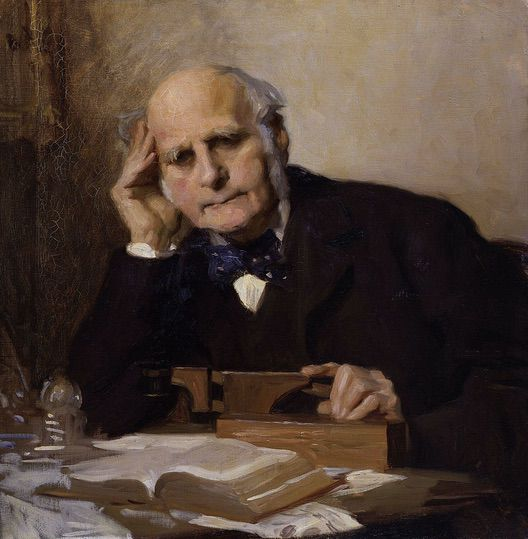
\includegraphics[width=0.8\linewidth]{images/supervised/linear_regression/francis_galton.jpg}
			\caption{Sir Francis Galton (1822 – 1911)}
%			\label{}
			\end{figure}

			\column{0.5\linewidth}
			\begin{figure}[!htbp]
				\centering
				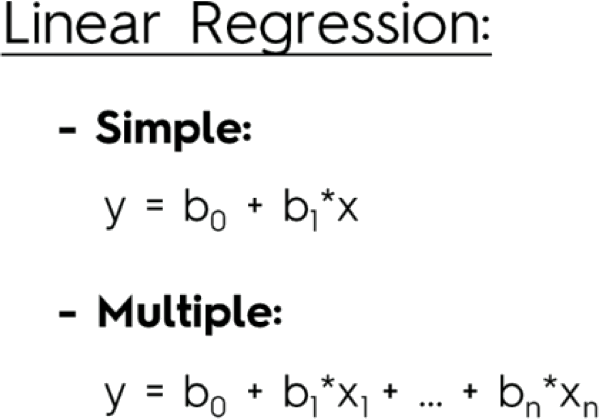
\includegraphics[width=0.85\linewidth]{images/supervised/linear_regression/linear_regression.png}
%			\caption{}
%			\label{}
			\end{figure}

	\end{columns}
\end{frame}


\begin{frame}

	\frametitle{Apprendimento supervisionato: training e loss}

	\begin{block}{Internamente un algoritmo di \ml supervisionato come valuta la scelta dei parametri in un modello parametrico?}
		Per entrare nel vivo del funzionamento degli algoritmi supervisionati nel Machine Learning:
		\begin{itemize}
			\item introduciamo il ``semplice'' algoritmo della \textbf{regressione lineare}
			\item introduciamo un possibile meccanismo secondo il quale potremmo andare a scegliere/modificare i parametri del modello (ad es \textbf{la discesa del gradiente})
			\item in modo tale da ottenere possibilmente la migliore risposta predittiva possibile (misurando la \textbf{loss})
		\end{itemize}
	\end{block}

\end{frame}


\begin{frame}

	\frametitle{La regressione lineare}

	\begin{block}{La regressione lineare}
		È noto da tempo che le cicale friniscono più frequentemente nei giorni più caldi rispetto ai giorni più freddi.
		\newlinedouble
		\pause
		Per decenni, scienziati professionisti e dilettanti hanno catalogato i dati sui frinii al minuto e sulla temperatura.
		\newlinedouble
		\pause
		Come regalo di compleanno, tua zia ti consegna il suo personale database e ti chiede di addestrare un modello a prevedere questa relazione, in modo che lei, contando il \textbf{numero di frinii al minuto}, possa d'ora in poi essere in grado di inferirne la \textbf{temperatura ambientale in gradi Celsius}.
	\end{block}

\end{frame}


\begin{frame}

	\frametitle{La regressione lineare}

	\begin{block}{}
		Utilizzando i dati, cerchiamo di esplorare questa relazione.\\
		Innanzitutto, esaminiamo i dati tracciandoli sul grafico.

		\begin{figure}[!htbp]
			\centering
			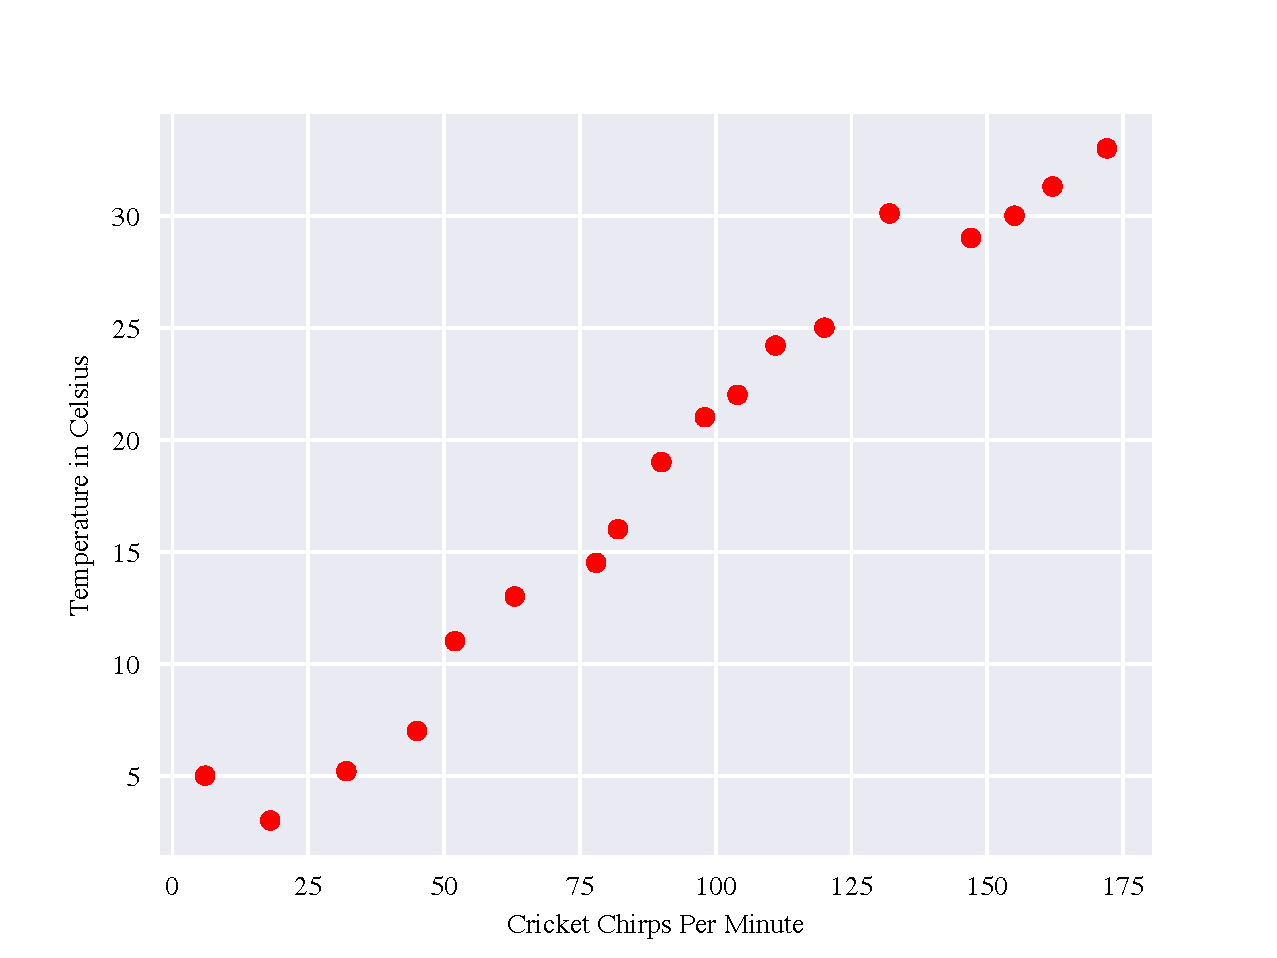
\includegraphics[width=7cm]{images/supervised/linear_regression/CricketPoints.pdf}
			%\caption{Stripe Radar for Fraud Detection}
		\end{figure}
		%Come previsto, il grafico mostra che la temperatura che aumenta con il numero di frinii.
	\end{block}

\end{frame}


\begin{frame}

	\frametitle{La regressione lineare}

	\begin{block}{}
		Questa relazione tra frinii e temperatura è lineare? Sì, allora puoi disegnare una singola linea retta come la seguente per approssimare questa relazione.

		\begin{figure}[!htbp]
			\centering
			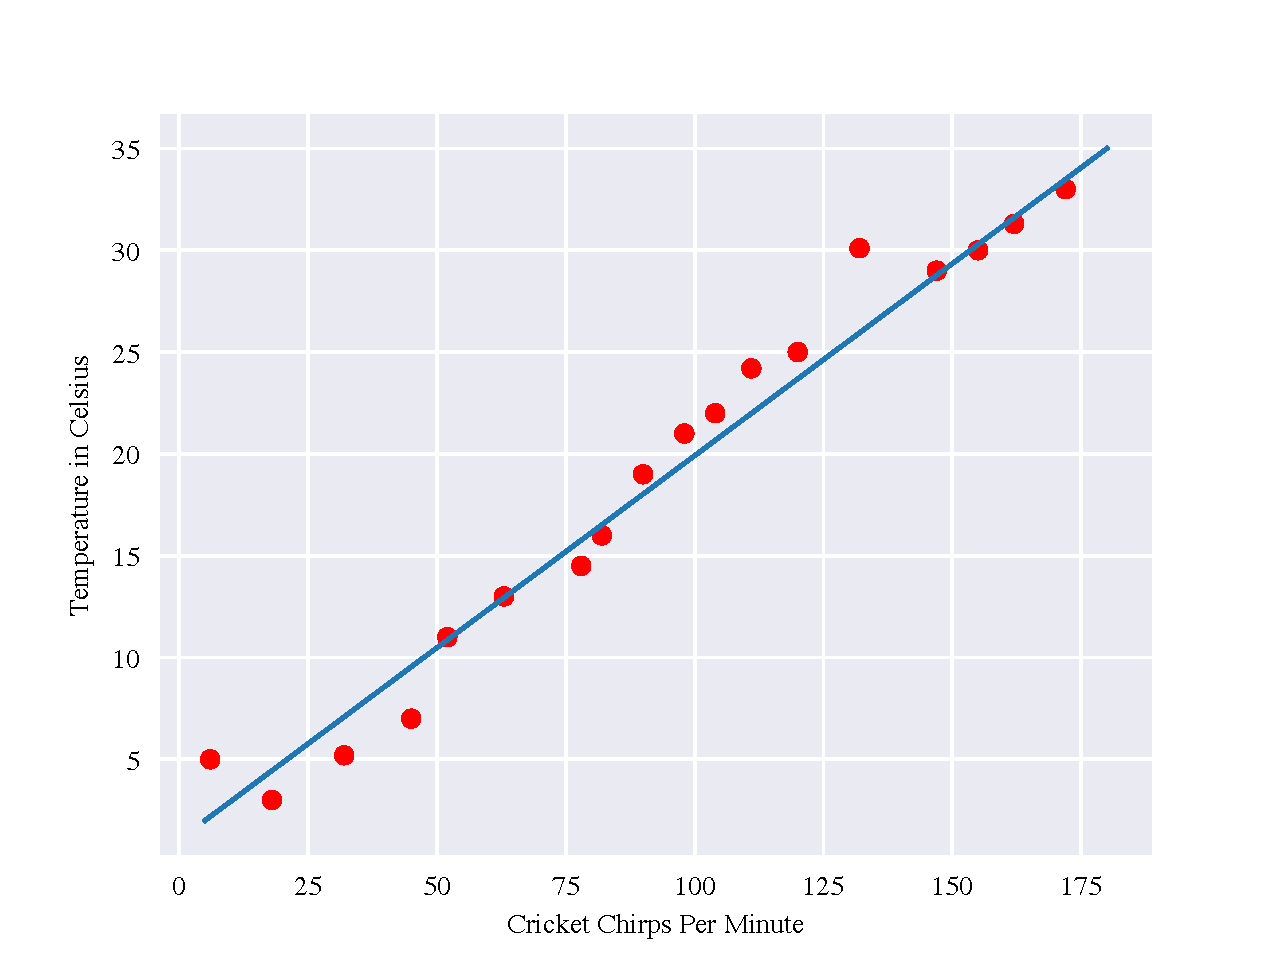
\includegraphics[width=7cm]{images/supervised/linear_regression/CricketLine.pdf}
			%\caption{Stripe Radar for Fraud Detection}
		\end{figure}
	\end{block}

\end{frame}


\begin{frame}

	\frametitle{La regressione lineare}

	\begin{block}{}
		È vero, la linea non passa attraverso ogni punto, ma mostra chiaramente  la relazione tra i frinii e temperatura.\\
		Utilizzando l'equazione di una retta, puoi scrivere questa relazione come segue:
		$$y = mx + b$$

		dove:

		\begin{itemize}
			\item $y$ è la temperatura in gradi Celsius, il valore che stiamo cercando di prevedere
			\item $m$ è la pendenza della linea
			\item $x$ è il numero di frinii al minuto, il valore della nostra funzione di input
			\item $b$ è l'\textit{y-intercept} (in italiano, l'\textit{intercetta})
		\end{itemize}
	\end{block}

\end{frame}


\begin{frame}

	\frametitle{La regressione lineare}

	\begin{block}{}
		Per convenzione nel Machine Learning, scriveremmo l'equazione per un modello in modo leggermente diverso:
		$$y' = b + \omega_1x_1$$

		dove:

		\begin{itemize}
			\item $y'$ è la temperatura in gradi Celsius, il valore che stiamo cercando di prevedere
			\item $b$ è il bias (l'\textit{y-intercept}), a volte indicato come $\omega_0$
			\item $\omega_1$ è il peso della $feature_1$. Il peso è lo stesso concetto della ``pendenza'' $m$ nell'equazione tradizionale di una retta
			\item $x_1$ è una feature (un input noto)
		\end{itemize}
	\end{block}

\end{frame}



\begin{frame}

	\frametitle{La regressione lineare}

	\begin{block}{}
		Per inferire (prevedere) la temperatura $y'$ per un nuovo valore di frinii al minuto $x_1$, è sufficiente sostituire il valore $x_1$ in questo modello.
		\newlinedouble
		Questo modello utilizza solo una feature.\\
		Un modello più sofisticato potrebbe fare affidamento su più features, ciascuna con un peso distinto ($\omega_1$, $\omega_2$, ecc.).
		\newlinedouble

		Ad esempio, un modello che si basa su tre features potrebbe essere:
		$$y' = b + \omega_1x_1 + \omega_2x_2 + \omega_3x_3$$
		\vspace{0.1mm}
	\end{block}

\end{frame}
